\section{Annexe}
\section{WENO-Z}
\subsubsection{Fifth order reconstruction, WENO5}\label{sssec:weno5}

\begin{figure}[H]
 \centering % avoid the use of \begin{center}...\end{center} and use \centering

 \includegraphics[width=\columnwidth]{stencil.png}
 \caption{Schematics illustrating the candidate stencils of seventh-order  TENO interpolation.}
 \label{fig:sample}
\end{figure}

\begin{equation}
\begin{aligned}
q_{i+1 / 2}^{l}=& w_{0}\left(\frac{1}{3} q_{i-2}-\frac{7}{6} q_{i-1}+\frac{11}{6} q_{i}\right) \\
&+w_{1}\left(-\frac{1}{6} q_{i-1}+\frac{5}{6} q_{i}+\frac{1}{3} q_{i+1}\right) \\
&+w_{2}\left(\frac{1}{3} q_{i}+\frac{5}{6} q_{i+1}-\frac{1}{6} q_{i+2}\right) \\
q_{i+1 / 2}^{R}=& w_{0}\left(\frac{1}{3} q_{i+1}+\frac{5}{6} q_{i}-\frac{1}{6} q_{i-1}\right) \\
&+w_{1}\left(-\frac{1}{6} q_{i+2}+\frac{5}{6} q_{i+1}+\frac{1}{3} q_{i}\right) \\
&+w_{2}\left(\frac{1}{3} q_{i+3}-\frac{7}{6} q_{i+2}+\frac{11}{6} q_{i+1}\right)
\end{aligned}
\end{equation}\\

$$d_0=\frac{1}{10} \quad d_1=\frac{3}{5} \quad d_2=\frac{3}{10}$$
\begin{equation}
\begin{array}{l}
w_{k}=\frac{\alpha_{k}}{\alpha_{0}+\alpha_{1}+\alpha_{2}}, \quad \alpha_{k}=d_k\left(1+\left(\frac{\tau_5}{\beta_{k}+\epsilon}\right)^2\right), \quad k=0,1,2\\
\end{array}
\end{equation}

\begin{equation}
\tau_5=\left|\beta_0-\beta_2\right|
\end{equation}

\begin{equation}
\begin{array}{l}
\beta_{0}=\frac{13}{12}\left(q_{i-2}-2 q_{i-1}+q_{i}\right)^{2}+\frac{1}{4}\left(q_{i-2}-4 q_{i-1}+3 q_{i}\right)^{2}\\
\beta_{1}=\frac{13}{12}\left(q_{i-1}-2 q_{i}+q_{i+1}\right)^{2}+\frac{1}{4}\left(q_{i-1}-q_{i+1}\right)^{2}\\
\beta_{2}=\frac{13}{12}\left(q_{i}-2 q_{i+1}+q_{i+2}\right)^{2}+\frac{1}{4}\left(3 q_{i}-4 q_{i+1}+q_{i+2}\right)^{2}
\end{array}
\end{equation}

$$d_0=\frac{3}{10} \quad d_1=\frac{3}{5} \quad d_2=\frac{1}{10}$$
\begin{equation}
\begin{array}{l}
w_{k}=\frac{\alpha_{k}}{\alpha_{0}+\alpha_{1}+\alpha_{2}}, \quad \alpha_{k}=d_k\left(1+\left(\frac{\tau_5}{\beta_{k}+\epsilon}\right)^2\right), \quad k=0,1,2\\
\end{array}
\end{equation}

\begin{equation}
\tau_5=\left|\beta_0-\beta_2\right|
\end{equation}

\begin{equation}
\begin{array}{l}
\beta_{0}=\frac{13}{12}\left(q_{i-1}-2 q_{i}+q_{i+1}\right)^{2}+\frac{1}{4}\left(q_{i-1}-4 q_{i}+3 q_{i+1}\right)^{2}\\
\beta_{1}=\frac{13}{12}\left(q_{i}-2 q_{i+1}+q_{i+2}\right)^{2}+\frac{1}{4}\left(q_{i}-q_{i+2}\right)^{2}\\
\beta_{2}=\frac{13}{12}\left(q_{i+1}-2 q_{i+2}+q_{i+3}\right)^{2}+\frac{1}{4}\left(3 q_{i+1}-4 q_{i+2}+q_{i+3}\right)^{2}
\end{array}
\end{equation}

\subsection{WENO-Z 7}
\begin{equation}
\begin{aligned}
q_{i+1 / 2}^{l}=& w_{0}\left(-\frac{1}{4} q_{i-3}+\frac{13}{12} q_{i-2}-\frac{23}{12} q_{i-1}+\frac{25}{12} q_{i}\right) \\
&+w_{1}\left(\frac{1}{12} q_{i-2}-\frac{5}{12} q_{i-1}+\frac{13}{12} q_{i}+\frac{1}{4} q_{i+1}\right) \\
&+w_{2}\left(-\frac{1}{12} q_{i-1}+\frac{7}{12} q_{i}+\frac{7}{12} q_{i+1}-\frac{1}{12} q_{i+2}\right) \\
&+w_{3}\left(\frac{1}{4} q_{i}+\frac{13}{12} q_{i+1}-\frac{5}{12} q_{i+2}+\frac{1}{12} q_{i+3}\right)
\end{aligned}
\end{equation}

\begin{equation}
\begin{aligned}
q_{i+1 / 2}^{R}=& w_{0}\left(\frac{1}{4} q_{i+1}+\frac{13}{12} q_{i}-\frac{5}{12} q_{i-1}+\frac{1}{12} q_{i-2}\right) \\
&+w_{1}\left(-\frac{1}{12} q_{i+2}+\frac{7}{12} q_{+1}+\frac{7}{12} q_{i}-\frac{1}{12} q_{i-1}\right) \\
&+w_{2}\left(\frac{1}{12} q_{i+3}-\frac{5}{12} q_{i+2}+\frac{13}{12} q_{i+1}+\frac{1}{4} q_{i}\right) \\
&+w_{3}\left(-\frac{1}{4} q_{i+4}+\frac{13}{12} q_{i+3}-\frac{23}{12} q_{i+2}+\frac{25}{12} q_{i+1}\right)
\end{aligned}
\end{equation}

$$d_0=\frac{1}{35} \quad d_1=\frac{12}{35} \quad d_2=\frac{18}{35} \quad d_3=\frac{4}{35}$$
\begin{equation}
\begin{array}{l}
w_{k}=\frac{\alpha_{k}}{\alpha_{0}+\alpha_{1}+\alpha_{2}}, \quad \alpha_{k}=d_k\left(1+\left(\frac{\tau_7}{\beta_{k}+\epsilon}\right)^2\right), \quad k=0,1,2\\
\end{array}
\end{equation}

\begin{equation}
\tau_7=\left|\beta_0+3\beta_1-3\beta_2-\beta3\right|
\end{equation}

\begin{equation}
\begin{aligned}
\beta_{0}=& q_{i-3}\left(547 q_{i-3}-3882 q_{i-2}+4642 q_{i-1}-1854 q_{i}\right) \\
&+q_{i-2}\left(7043 q_{i-2}-17246 q_{i-1}+7042 q_{i}\right) \\
&+q_{i-1}\left(11003 q_{i-1}-9402 q_{i}\right)+q_{i}\left(2107 q_{i}\right)
\end{aligned}
\end{equation}

\begin{equation}
\begin{aligned}
\beta_{1}=& q_{i-2}\left(267 q_{i-2}-1642 q_{i-1}+1602 q_{i}-494 q_{i+1}\right) \\
&+q_{i-1}\left(2843 q_{i-1}-5966 q_{i}+1922 q_{i+1}\right)\\
&+q_{i}\left(3443 q_{i}-2522 q_{i+1}\right)+q_{i+1}\left(547 q_{i+1}\right)
\end{aligned}
\end{equation}

\begin{equation}
\begin{aligned}
\beta_{2}=& q_{i-1}\left(547 q_{i-1}-2522 q_{i}+1922 q_{i+1}-494 q_{i+2}\right) \\
&+q_{i}\left(3443 q_{i}-5966 q_{i+1}+1602 q_{i+2}\right) \\
&+q_{i+1}\left(2843 q_{i+1}-1642 q_{i+2}\right)+q_{i+2}\left(267 q_{i+2}\right)
\end{aligned}
\end{equation}

\begin{equation}
\begin{aligned}
\beta_{3}=& q_{i}\left(2107 q_{i}-9402 q_{i+1}+7042 q_{i+2}-1854 q_{i+3}\right) \\
&+q_{i+1}\left(11003 q_{i+1}-17246 q_{i+2}+4642 q_{i+3}\right) \\
&+q_{i+2}\left(7043 q_{i+2}-3882 q_{i+3}\right)+q_{i+3}\left(547 q_{i+3}\right)
\end{aligned}
\end{equation}

$$d_0=\frac{4}{35} \quad d_1=\frac{18}{35} \quad d_2=\frac{12}{35} \quad d_3=\frac{1}{35}$$
\begin{equation}
\begin{array}{l}
w_{k}=\frac{\alpha_{k}}{\alpha_{0}+\alpha_{1}+\alpha_{2}}, \quad \alpha_{k}=d_k\left(1+\left(\frac{\tau_7}{\beta_{k}+\epsilon}\right)^2\right), \quad k=0,1,2\\
\end{array}
\end{equation}

\begin{equation}
\tau_7=\left|\beta_0+3\beta_1-3\beta_2-\beta3\right|
\end{equation}

\begin{equation}
\begin{aligned}
\beta_{0}=& q_{i-2}\left(547 q_{i-2}-3882 q_{i-1}+4642 q_{i}-1854 q_{i+1}\right) \\
&+q_{i-1}\left(7043 q_{i-1}-17246 q_{i}+7042 q_{+1}\right) \\
&+q_{i}\left(11003 q_{i}-9402 q_{i+1}\right)+q_{i+1}\left(2107 q_{i+1}\right)
\end{aligned}
\end{equation}

\begin{equation}
\begin{aligned}
\beta_{1}=& q_{i-1}\left(267 q_{i-1}-1642 q_{i}+1602 q_{i+1}-494 q_{i+2}\right) \\
&+q_{i}\left(2843 q_{i}-5966 q_{i+1}+1922 q_{i+2}\right)\\
&+q_{i+1}\left(3443 q_{i+1}-2522 q_{i+2}\right)+q_{i+2}\left(547 q_{i+2}\right)
\end{aligned}
\end{equation}

\begin{equation}
\begin{aligned}
\beta_{2}=& q_{i}\left(547 q_{i}-2522 q_{i+1}+1922 q_{i+2}-494 q_{i+3}\right) \\
&+q_{i+1}\left(3443 q_{i+1}-5966 q_{i+2}+1602 q_{i+3}\right) \\
&+q_{i+2}\left(2843 q_{i+2}-1642 q_{i+3}\right)+q_{i+3}\left(267 q_{i+3}\right)
\end{aligned}
\end{equation}

\begin{equation}
\begin{aligned}
\beta_{3}=& q_{i+1}\left(2107 q_{i+1}-9402 q_{i+2}+7042 q_{i+3}-1854 q_{i+4}\right) \\
&+q_{i+2}\left(11003 q_{i+2}-17246 q_{i+3}+4642 q_{i+4}\right) \\
&+q_{i+3}\left(7043 q_{i+3}-3882 q_{i+4}\right)+q_{i+34}\left(547 q_{i+4}\right)
\end{aligned}
\end{equation}


\subsection{TENO reconstruction schemes}

\subsubsection{Fifth order reconstruction, TENO5}

\begin{equation}
\begin{aligned}
q_{i+1 / 2}^{l}=& w_{0}\left(-\frac{1}{6} q_{i-1}+\frac{5}{6} q_{i}+\frac{2}{6} q_{i+1}\right) \\
&+w_{1}\left(\frac{2}{6} q_{i}+\frac{5}{6} q_{i+1}-\frac{1}{6} q_{i+2}\right) \\
&+w_{2}\left(\frac{2}{6} q_{i-2}-\frac{7}{6} q_{i-1}+\frac{11}{6} q_{i}\right) \\
\end{aligned}
\end{equation}

\begin{equation}
\begin{array}{l}
\beta_{0}=\frac{13}{12}\left(q_{i-1}-2 q_{i}+q_{i+1}\right)^{2}+\frac{1}{4}\left(q_{i-1}-q_{i+1}\right)^{2}\\
\beta_{1}=\frac{13}{12}\left(q_{i}-2 q_{i+1}+q_{i+2}\right)^{2}+\frac{1}{4}\left(3 q_{i}-4 q_{i+1}+q_{i+2}\right)^{2}\\
\beta_{2}=\frac{13}{12}\left(q_{i-2}-2 q_{i-1}+q_{i}\right)^{2}+\frac{1}{4}\left(q_{i-2}-4 q_{i-1}+3 q_{i}\right)^{2}\\
\end{array}
\end{equation}

\begin{equation}
\gamma_{k}=\left(1+\frac{\tau_{5}}{\beta_{k}+\varepsilon}\right)^{2}, k=0, \ldots, 2
\end{equation}

\begin{equation}
\tau_{5}=\left|\beta_{5}-\frac{1}{6}\left(\beta_{1}+\beta_{2}+4 \beta_{0}\right)\right|=O\left(\Delta x^{6}\right)
\end{equation}

\begin{equation}
\begin{aligned}
\beta_{5}&=\frac{1727}{1260}q_{i-2}^2+(67923q_i -51001q_{i-1} -38947q_{i+1}+8209q_{i+2})\frac{q_{i-2}}{5040}\\
&+\frac{104963}{5040}q_{i-1}^2+(-299076q_{i}+179098q_{i+1}-38947q_{i+2})\frac{q_{i-1}}{5040}\\
&+\frac{104963}{5040}q_{i+1}^2+(-299076q_{i}-51001q_{i+2})\frac{q_{i+1}}{5040}\\
&+\frac{77051}{1680}q_{i}^2+\frac{7547}{560}q_{i+2}q_{i}+\frac{1727}{1260}q_{i+2}^2
\end{aligned}
\end{equation}
% cg2 = 0.1727e4 / 0.1260e4 * pow(f_(i - 2), 2) + (67923 * f_i - 51001 * f_(i - 1) - 38947 * f_(i + 1) + 8209 * f_(i + 2)) * f_(i - 2) / 5040 + 0.104963e6 / 0.5040e4 * (int) pow((double) f_(i - 1), (double) 2) + (-299076 * f_i + 179098 * f_(i + 1) - 38947 * f_(i + 2)) * f_(i - 1) / 5040 + 0.104963e6 / 0.5040e4 * (int) pow((double) f_(i + 1), (double) 2) + (-299076 * f_i - 51001 * f_(i + 2)) * f_(i + 1) / 5040 + 0.77051e5 / 0.1680e4 * f_i * f_i + 0.7547e4 / 0.560e3 * f_(i + 2) * f_i + 0.1727e4 / 0.1260e4 * (int) pow((double) f_(i + 2), (double) 2);
\begin{equation}
\chi_{k}=\frac{\gamma_{k}}{\sum_{k=0}^{2} \gamma_{k}}
\end{equation}

\begin{equation}
\delta_{k}=\left\{\begin{array}{ll}
0, & \text { if } \chi_{k}<C_{T} \\
1, & \text { otherwise }
\end{array}\right.
\end{equation}

$$d_0=\frac{6}{10} \quad d_1=\frac{3}{10} \quad d_2=\frac{1}{10}$$
\begin{equation}
\begin{array}{l}
w_{k}=\frac{\alpha_{k}}{\sum_{k=0}^{2} \alpha_{k}}, \quad \alpha_{k}=d_k\delta_k, \quad k=0,1,2\\
\end{array}
\end{equation}

\begin{equation}
\begin{aligned}
q_{i+1 / 2}^{r}=& w_{0}\left(\frac{2}{6} q_{i}+\frac{5}{6} q_{i+1}-\frac{1}{6} q_{i+2}\right) \\
&+w_{1}\left(-\frac{1}{6} q_{i-1}+\frac{5}{6} q_{i}+\frac{2}{6} q_{i+1}\right) \\
&+w_{2}\left(\frac{11}{6} q_{i+1}-\frac{7}{6} q_{i+2}+\frac{2}{6} q_{i+3}\right) \\
\end{aligned}
\end{equation}

\begin{equation}
\begin{array}{l}
\beta_{0}=\frac{13}{12}\left(q_{i}-2 q_{i+1}+q_{i+2}\right)^{2}+\frac{1}{4}\left(q_{i}-q_{i+2}\right)^{2}\\
\beta_{1}=\frac{13}{12}\left(q_{i-1}-2 q_{i}+q_{i+1}\right)^{2}+\frac{1}{4}\left(q_{i-1}-4 q_{i}+q_{i+1}\right)^{2}\\
\beta_{2}=\frac{13}{12}\left(q_{i+1}-2 q_{i+2}+q_{i+3}\right)^{2}+\frac{1}{4}\left(3q_{i+1}-4 q_{i+2}+q_{i+3}\right)^{2}\\
\end{array}
\end{equation}

\begin{equation}
\gamma_{k}=\left(1+\frac{\tau_{5}}{\beta_{k}+\varepsilon}\right)^{2}, k=0, \ldots, 2
\end{equation}

\begin{equation}
\tau_{5}=\left|\beta_{5}-\frac{1}{6}\left(\beta_{1}+\beta_{2}+4 \beta_{0}\right)\right|=O\left(\Delta x^{6}\right)
\end{equation}

\begin{equation}
\begin{aligned}
\beta_{5}&=\frac{1727}{1260}q_{i-1}^2+(-51001q_{i}+67923q_{i+1} -38947q_{i+2}+8209q_{i+3})\frac{q_{i-1}}{5040}\\
&+\frac{77051}{1680}q_{i+1}^2+(-299076q_{i}-299076q_{i+2}+67923q_{i+3})\frac{q_{i+1}}{5040}\\
&+\frac{104963}{5040}q_{i+2}^2+(179098q_{i}-51001q_{i+3})\frac{q_{i+2}}{5040}\\
&+\frac{104963}{5040}q_{i}^2-\frac{38947}{5040}q_{i+3}q_{i}+\frac{1727}{1260}q_{i+3}^2
\end{aligned}
\end{equation}
% cg6 = 0.1727e4 / 0.1260e4 * pow(f_(i - 1), 2) + (-51001 * f_i + 67923 * f_(i + 1) - 38947 * f_(i + 2) + 8209 * f_(i + 3)) * f_(i - 1) / 5040 + 0.77051e5 / 0.1680e4 * (int) pow((double) f_(i + 1), (double) 2) + (-299076 * f_i - 299076 * f_(i + 2) + 67923 * f_(i + 3)) * f_(i + 1) / 5040 + 0.104963e6 / 0.5040e4 * (int) pow((double) f_(i + 2), (double) 2) + (179098 * f_i - 51001 * f_(i + 3)) * f_(i + 2) / 5040 + 0.104963e6 / 0.5040e4 * f_i * f_i - 0.38947e5 / 0.5040e4 * f_(i + 3) * f_i + 0.1727e4 / 0.1260e4 * (int) pow((double) f_(i + 3), (double) 2);
\begin{equation}
\chi_{k}=\frac{\gamma_{k}}{\sum_{k=0}^{2} \gamma_{k}}
\end{equation}

\begin{equation}
\delta_{k}=\left\{\begin{array}{ll}
0, & \text { if } \chi_{k}<C_{T} \\
1, & \text { otherwise }
\end{array}\right.
\end{equation}

$$d_0=\frac{6}{10} \quad d_1=\frac{3}{10} \quad d_2=\frac{1}{10}$$
\begin{equation}
\begin{array}{l}
w_{k}=\frac{\alpha_{k}}{\sum_{k=0}^{2} \alpha_{k}}, \quad \alpha_{k}=d_k\delta_k, \quad k=0,1,2\\
\end{array}
\end{equation}

\subsubsection{Seventh order reconstruction, TENO7}

\begin{equation}
\begin{aligned}
q_{i+1 / 2}^{l}=& w_{0}\left(-\frac{1}{6} q_{i-1}+\frac{5}{6} q_{i}-\frac{2}{6} q_{i+1}\right) \\
&+w_{1}\left(\frac{2}{6} q_{i}+\frac{5}{6} q_{i+1}-\frac{1}{6} q_{i+2}\right) \\
&+w_{2}\left(\frac{2}{6} q_{i-2}-\frac{7}{6} q_{i-1}+\frac{11}{6} q_{i}\right) \\
&+w_{3}\left(\frac{3}{12} q_{i}+\frac{13}{12} q_{i+1}-\frac{5}{12} q_{i+2}+\frac{1}{12}q_{i+3}\right) \\
&+w_{4}\left(-\frac{3}{12} q_{i-3}+\frac{13}{12} q_{i-2}-\frac{23}{12} q_{i-1}+\frac{25}{12}q_{i}\right) \\
\end{aligned}
\end{equation}

\begin{equation}
\begin{aligned}
\beta_{0}&=\frac{13}{12}\left(q_{i-1}-2 q_{i}+q_{i+1}\right)^{2}+\frac{1}{4}\left(q_{i-1}-q_{i+1}\right)^{2}\\
\beta_{1}&=\frac{13}{12}\left(q_{i}-2 q_{i+1}+q_{i+2}\right)^{2}+\frac{1}{4}\left(3 q_{i}-4 q_{i+1}+q_{i+2}\right)^{2}\\
\beta_{2}&=\frac{13}{12}\left(q_{i-2}-2 q_{i-1}+q_{i}\right)^{2}+\frac{1}{4}\left(q_{i-2}-4 q_{i-1}+3 q_{i}\right)^{2}\\
\beta_{3} &=\frac{1}{240}\left[q_{i}\left(2107 q_{i}-9402 q_{i+1}+7042 q_{i+2}-1854 q_{i+3}\right)\right.\\
&+q_{i+1}\left(11003 q_{i+1}-17246 q_{i+2}+4642 q_{i+3}\right) \\
&\left.+q_{i+2}\left(7043 q_{i+2}-3882 q_{i+3}\right)+547 q_{i+3} q_{i+3}\right] \\
\beta_{4} &=\frac{1}{240}\left[q_{i-3}\left(547 q_{i-3}-3882 q_{i-2}+4642 q_{i-1}-1854 q_{i}\right)\right.\\
&+q_{i-2}\left(7043 q_{i-2}-17246 q_{i-1}+7042 q_{i}\right) \\
&\left.+q_{i-1}\left(11003 q_{i-1}-9402 q_{i}\right)+2107 q_{i} q_{i}\right]
\end{aligned}
\end{equation}

\begin{equation}
\gamma_{k}=\left(1+\frac{\tau_{7}}{\beta_{k}+\varepsilon}\right)^{2}, k=0, \ldots, 4
\end{equation}

\begin{equation}
\tau_{7}=\left|\beta_{7}-\frac{1}{6}\left(\beta_{1}+\beta_{2}+4 \beta_{0}\right)\right|=O\left(\Delta x^{6}\right)
\end{equation}

\begin{equation}
\begin{aligned}
\beta_7&=\frac{2627203}{1871100}q_{i - 2}^2 + (2283428883q_{i} - 969999969 q_{i - 1} - 2806252532 q_{i + 1} + 1902531828 q_{i + 2} - 676871859 q_{i + 3} + 99022657 q_{i + 4}) \frac{q_{i - 2}}{59875200}\\
&+ \frac{108444169}{2217600}q_{i - 1}^2 + (-14296379553  q_{i} + 18083339772 q_{i + 1} - 12546315963 q_{i + 2} + 4550242446 q_{i + 3} - 676871859  q_{i + 4}) \frac{q_{i - 1}}{59875200}\\
&+ \frac{1607739169}{2993760} q_{i + 1}^2 + (-47431870620  q_{i} - 47431870620 q_{i + 2} + 18083339772 q_{i + 3} - 2806252532  q_{i + 4})\frac{q_{i + 1}}{59875200} \\
&+ \frac{16790707}{55440} q_{i + 2}^2 (33820678305 q_{i} - 14296379553 q_{i + 3} + 2283428883 q_{i + 4}) \frac{q_{i + 2}}{59875200}\\
&+ \frac{108444169}{2217600} q_{i + 3}^2 + (-12546315963 q_{i} - 969999969 q_{i + 4})\frac{q_{i + 3}}{59875200}\\
&+ \frac{16790707}{55440}q_{i}^2 + \frac{158544319}{4989600} q_{i + 4} q_{i} +\frac{2627203}{1871100} q_{i + 4}^2;
\end{aligned}
\end{equation}
%cg7 = 0.2627203e7 / 0.1871100e7 * pow(f_(i - 2), 2) + (2283428883 * f_i - 969999969 * f_(i - 1) - 2806252532 * f_(i + 1) + 1902531828 * f_(i + 2) - 676871859 * f_(i + 3) + 99022657 * f_(i + 4)) * f_(i - 2) / 59875200 + 0.108444169e9 / 0.2217600e7 * (int) pow((double) f_(i - 1), (double) 2) + (-14296379553 * f_i + 18083339772 * f_(i + 1) - 12546315963 * f_(i + 2) + 4550242446 * f_(i + 3) - 676871859 * f_(i + 4)) * f_(i - 1) / 59875200 + 0.1607739169e10 / 0.2993760e7 * (int) pow((double) f_(i + 1), (double) 2) + (-47431870620 * f_i - 47431870620 * f_(i + 2) + 18083339772 * f_(i + 3) - 2806252532 * f_(i + 4)) * f_(i + 1) / 59875200 + 0.16790707e8 / 0.55440e5 * (int) pow((double) f_(i + 2), (double) 2) + (33820678305 * f_i - 14296379553 * f_(i + 3) + 2283428883 * f_(i + 4)) * f_(i + 2) / 59875200 + 0.108444169e9 / 0.2217600e7 * (int) pow((double) f_(i + 3), (double) 2) + (-12546315963 * f_i - 969999969 * f_(i + 4)) * f_(i + 3) / 59875200 + 0.16790707e8 / 0.55440e5 * f_i * f_i + 0.158544319e9 / 0.4989600e7 * f_(i + 4) * f_i + 0.2627203e7 / 0.1871100e7 * (int) pow((double) f_(i + 4), (double) 2);
\begin{equation}
\chi_{k}=\frac{\gamma_{k}}{\sum_{k=0}^{4} \gamma_{k}}
\end{equation}

\begin{equation}
\delta_{k}=\left\{\begin{array}{ll}
0, & \text { if } \chi_{k}<C_{T} \\
1, & \text { otherwise }
\end{array}\right.
\end{equation}

$$d_0=\frac{18}{35} \quad d_1=\frac{9}{35} \quad d_2=\frac{3}{35} \quad d_3=\frac{4}{35} \quad d_4=\frac{1}{35}$$
\begin{equation}
\begin{array}{l}
w_{k}=\frac{\alpha_{k}}{\sum_{k=0}^{4} \alpha_{k}}, \quad \alpha_{k}=d_k\delta_k, \quad k=0,1,2,3,4\\
\end{array}
\end{equation}


\begin{equation}
\begin{aligned}
q_{i+1 / 2}^{r}=& w_{0}\left(\frac{2}{6} q_{i}+\frac{5}{6} q_{i+1}-\frac{1}{6} q_{i+2}\right) \\
&+w_{1}\left(-\frac{1}{6} q_{i-1}+\frac{5}{6} q_{i}+\frac{2}{6} q_{i+1}\right) \\
&+w_{2}\left(\frac{11}{6} q_{i+1}-\frac{7}{6} q_{i+2}+\frac{2}{6} q_{i+3}\right) \\
&+w_{3}\left(\frac{1}{12} q_{i-2}-\frac{5}{12} q_{i-1}+\frac{13}{12} q_{i}+\frac{3}{12}q_{i+1}\right) \\
&+w_{4}\left(\frac{25}{12} q_{i+1}-\frac{23}{12} q_{i+2}+\frac{13}{12} q_{i+3}-\frac{3}{12}q_{i+4}\right) \\
\end{aligned}
\end{equation}

\begin{equation}
\begin{aligned}
\beta_{0}&=\frac{13}{12}\left(q_{i}-2 q_{i+1}+q_{i+2}\right)^{2}+\frac{1}{4}\left(q_{i}-q_{i+2}\right)^{2}\\
\beta_{1}&=\frac{13}{12}\left(q_{i-1}-2 q_{i}+q_{i+1}\right)^{2}+\frac{1}{4}\left(q_{i-1}-4 q_{i}+q_{i+1}\right)^{2}\\
\beta_{2}&=\frac{13}{12}\left(q_{i+1}-2 q_{i+2}+q_{i+3}\right)^{2}+\frac{1}{4}\left(3q_{i+1}-4 q_{i+2}+q_{i+3}\right)^{2}\\
\beta_{3} &=\frac{1}{240}\left[q_{i+1}\left(2107 q_{i+1}-9402 q_{i}+7042 q_{i-1}-1854 q_{i-2}\right)\right.\\
&+q_{i}\left(11003 q_{i}-17246 q_{i-1}+4642 q_{i-2}\right) \\
&\left.+q_{i-1}\left(7043 q_{i-1}-3882 q_{i-2}\right)+547 q_{i-2} q_{i-2}\right] \\
\beta_{4} &=\frac{1}{240}\left[q_{i+4}\left(547 q_{i+4}-3882 q_{i+3}+4642 q_{i+2}-1854 q_{i+1}\right)\right.\\
&+q_{i+3}\left(7043 q_{i+3}-17246 q_{i+2}+7042 q_{i+1}\right) \\
&\left.+q_{i+2}\left(11003 q_{i+2}-9402 q_{i+1}\right)+2107 q_{i+1} q_{i+1}\right]
\end{aligned}
\end{equation}

\begin{equation}
\gamma_{k}=\left(1+\frac{\tau_{7}}{\beta_{k}+\varepsilon}\right)^{2}, k=0, \ldots, 4
\end{equation}

\begin{equation}
\tau_{7}=\left|\beta_{7}-\frac{1}{6}\left(\beta_{1}+\beta_{2}+4 \beta_{0}\right)\right|=O\left(\Delta x^{6}\right)
\end{equation}

\begin{equation}
\begin{aligned}
\beta_7&=\frac{2627203}{1871100}q_{i - 3}^2 + (2283428883q_{i-1} - 969999969 q_{i - 2} - 2806252532 q_{i} + 1902531828 q_{i + 1} - 676871859 q_{i + 2} + 99022657 q_{i + 3}) \frac{q_{i - 3}}{59875200}\\
&+ \frac{108444169}{2217600}q_{i - 2}^2 + (-14296379553  q_{i-1} + 18083339772 q_{i} - 12546315963 q_{i + 1} + 4550242446 q_{i + 2} - 676871859  q_{i + 3}) \frac{q_{i - 2}}{59875200}\\
&+ \frac{1607739169}{55440} q_{i- 1}^2 + (-47431870620  q_{i} + 33820678305 q_{i + 1} -12546315963 q_{i + 2} + 1902531828  q_{i + 3})\frac{q_{i - 1}}{59875200} \\
&+ \frac{16790707}{55440} q_{i + 1}^2 (-47431870620 q_{i} - 14296379553 q_{i + 2} + 2283428883 q_{i + 3}) \frac{q_{i + 1}}{59875200}\\
&+ \frac{108444169}{2217600} q_{i + 2}^2 + (18083339772 q_{i} - 969999969 q_{i + 3})\frac{q_{i + 3}}{59875200}\\
&+ \frac{16790707}{2993760}q_{i}^2 - \frac{701563133}{14968800} q_{i + 3} q_{i} +\frac{2627203}{1871100} q_{i + 3}^2;
\end{aligned}
\end{equation}
%cg5 = 0.2627203e7 / 0.1871100e7 * pow(f_(i - 3), 2) + (-2806252532 * f_i - 969999969 * f_(i - 2) + 2283428883 * f_(i - 1) + 1902531828 * f_(i + 1) - 676871859 * f_(i + 2) + 99022657 * f_(i + 3)) * f_(i - 3) / 59875200 + 0.108444169e9 / 0.2217600e7 * (int) pow((double) f_(i - 2), (double) 2) + (18083339772 * f_i - 14296379553 * f_(i - 1) - 12546315963 * f_(i + 1) + 4550242446 * f_(i + 2) - 676871859 * f_(i + 3)) * f_(i - 2) / 59875200 + 0.16790707e8 / 0.55440e5 * (int) pow((double) f_(i - 1), (double) 2) + (-47431870620 * f_i + 33820678305 * f_(i + 1) - 12546315963 * f_(i + 2) + 1902531828 * f_(i + 3)) * f_(i - 1) / 59875200 + 0.16790707e8 / 0.55440e5 * (int) pow((double) f_(i + 1), (double) 2) + (-47431870620 * f_i - 14296379553 * f_(i + 2) + 2283428883 * f_(i + 3)) * f_(i + 1) / 59875200+ 0.108444169e9 / 0.2217600e7 * (int) pow((double) f_(i + 2), (double) 2) + (18083339772 * f_i - 969999969 * f_(i + 3)) * f_(i + 2) / 59875200 + 0.1607739169e10 / 0.2993760e7 * f_i * f_i - 0.701563133e9 / 0.14968800e8 * f_(i + 3) * f_i + 0.2627203e7 / 0.1871100e7 * (int) pow((double) f_(i + 3), (double) 2);
\begin{equation}
\chi_{k}=\frac{\gamma_{k}}{\sum_{k=0}^{4} \gamma_{k}}
\end{equation}

\begin{equation}
\delta_{k}=\left\{\begin{array}{ll}
0, & \text { if } \chi_{k}<C_{T} \\
1, & \text { otherwise }
\end{array}\right.
\end{equation}

$$d_0=\frac{18}{35} \quad d_1=\frac{9}{35} \quad d_2=\frac{3}{35} \quad d_3=\frac{4}{35} \quad d_4=\frac{1}{35}$$
\begin{equation}
\begin{array}{l}
w_{k}=\frac{\alpha_{k}}{\sum_{k=0}^{4} \alpha_{k}}, \quad \alpha_{k}=d_k\delta_k, \quad k=0,1,2,3,4\\
\end{array}
\end{equation}

\subsection{Approximate Riemann solvers}


\subsubsection{HLL solver}\label{sssec:HLL}

\begin{equation}
\tilde{a}=\sqrt{(\gamma-1)\left[\widetilde{H}-\frac{1}{2}\left(\tilde{u}^{2}+\tilde{v}^{2}\right)\right]}
\end{equation}

\begin{equation}
\tilde{u}=\frac{u_{R} \sqrt{\rho_{R}}+u_{L} \sqrt{\rho_{L}}}{\sqrt{\rho_{R}}+\sqrt{\rho_{L}}}
\end{equation}

\begin{equation}
\bar{v}=\frac{v_{R} \sqrt{\rho_{R}}+v_{L} \sqrt{\rho_{L}}}{\sqrt{\rho_{R}}+\sqrt{\rho_{L}}}
\end{equation}

\begin{equation}
\widetilde{H}=\frac{H_{R} \sqrt{\rho_{R}}+H_{L} \sqrt{\rho_{L}}}{\sqrt{\rho_{R}}+\sqrt{\rho_{L}}}
\end{equation}

\begin{equation}
\begin{array}{l}
\mathbf{S}_{R}=\max \left((u_{L}-a_{L}),(u_{L}+a_{L}),(u_{R}-a_{R}),(u_{R}+a_{R})\right) \\
\mathbf{S}_{L}=-\mathbf{S}_{R}
\end{array}
\end{equation}

\begin{equation}
\mathbf{F}_{i+1 / 2}=\left\{\begin{array}{ll}
\mathbf{F}^{L}, & \text { if } \quad S_{L} \geqslant 0 \\
\mathbf{F}^{R}, & \text { if } \quad S_{R} \leqslant 0 \\
\frac{S_{R} F^{L}-S_{L} F^{R}+S_{L} S_{R}\left(q_{i+1 / 2}^{R}-q_{i+1 / 2}^{\perp}\right)}{S_{R}-S_{L}}, & \text { otherwise. }
\end{array}\right.
\end{equation}

\subsubsection{HLLC solver}\label{sssec:HLLC}
\begin{equation}
\begin{array}{l}
\mathbf{S}_{R}=\max \left((u_{R}-a_{R}),(u_{R}+a_{R})\right) \\
\mathbf{S}_{L}=\min \left((u_{L}-a_{L}),(u_{L}+a_{L})\right)\\
\mathbf{S}_{*}=\frac{p_L-p_R-\rho_L u_L(S_L-u_L)+\rho_R u_R(S_R-u_R)}{\rho_L u_L-\rho_Ru_R+\rho_R S_R-\rho_L S_L}
\end{array}
\end{equation}

\begin{equation}
\mathbf{p_*}=\rho_r(u_R-S_R)(u_R-S_*)+p_R
\end{equation}

\begin{equation}
\begin{array}{l}
\mathbf{F_*}_{L}=\mathbf{F}_{L}+S_{L}\left(\mathbf{U}_{* L}-\mathbf{U}_{L}\right),\\
\mathbf{F_*}_{R}=\mathbf{F}_{R}+S_{R}\left(\mathbf{U}_{* R}-\mathbf{U}_{R}\right),
\end{array}
\end{equation}

\begin{equation}
\mathbf{F}_{i+\frac{1}{2}}^{HLLC}=\left\{\begin{array}{l}
\mathbf{F}_{L}, \text { if } 0 \leq S_{L} \\
\mathbf{F}_{* L}, \text { if } S_{L} \leq 0 \leq S_{*} \\
\mathbf{F}_{* R}, \text { if } S_{*} \leq 0 \leq S_{R} \\
\mathbf{F}_{R}, \text { if } \quad 0 \geq S_{R}
\end{array}\right.
\end{equation}

\subsubsection{AUSM-up solver}

$$
\begin{array}{ll}
\tilde{p}=\left.f_{p}^{+}\right|_{z} p_{L}+\left.f_{p}^{-}\right|_{z} p_{R}+p_{u} & \\
\left.f_{p}^{\pm}\right|_{z}=\left\{\begin{array}{ll}
\frac{1}{2}(1 \pm \operatorname{sign}(M)), & \text { if }|M| \geqslant 1 \\
\frac{1}{4}(M \pm 1)^{2}(2 \mp M) \pm \alpha M\left(M^{2}-1\right)^{2}, & \text { otherwise }
\end{array}\right. \\
p_{u}=-K_{u} \beta_{+} \beta_{-}\left(\rho_{L}+\rho_{R}\right)\left(f_{a} c_{1 / 2}\right)\left(V_{n}^{-}-V_{n}^{+}\right)
\end{array}
$$
where $c_{1 / 2}$ is calculated as
$$
\begin{array}{l}
c_{1 / 2}=\min \left(\tilde{c}_{l}, \tilde{c}_{R}\right), \quad \tilde{c}_{L}=c^{-2} / \max \left(c^{*}, V_{n}^{+}\right), \quad \tilde{c}_{R}=c^{* 2} / \max \left(c^{*},-V_{n}^{-}\right) \\
c^{* 2}=\frac{2(\gamma-1)}{(\gamma+1)} H
\end{array}
$$

\subsubsection{Slau2 solver}
$$
\begin{array}{l}
\mathbf{F}_{1 / 2}=\frac{\dot{m}+|\dot{m}|}{2} \Psi^{+}+\frac{\dot{m}-|\dot{m}|}{2} \Psi^{-}+\tilde{p} \mathbf{N} \\
\Psi=(1, u, v, w, H)^{T}, \quad \mathbf{N}=\left(0, n_{x}, n_{y}, n_{z}, 0\right)^{\top}
\end{array}
$$

$$
\begin{array}{l}
\tilde{p}=\frac{p_{\mathrm{L}}+p_{R}}{2}+\frac{f_{p}^{+}-f_{p}^{-}}{2}\left(p_{L}-p_{R}\right)+\frac{1}{c_{1 / 2}} \sqrt{\frac{u_{L}^{2}+v_{l}^{2}+w_{L}^{2}+u_{R}^{2}+v_{R}^{2}+w_{R}^{2}}{2}}\left(f_{p}^{+}+f_{p}^{-}-1\right) \frac{p_{l}+p_{R}}{2}
\end{array}
$$
Considering possible extension to real fluids [30] , the above expression is improved further:
$$
\begin{array}{l}
\tilde{p}=\frac{p_{L}+p_{R}}{2}+\frac{f_{p}^{+}-f_{p}^{-}}{2}\left(p_{l}-p_{R}\right)+\sqrt{\frac{u_{l}^{2}+v_{l}^{2}+w_{l}^{2}+u_{R}^{2}+v_{R}^{2}+w_{R}^{2}}{2}}\left(f_{p}^{+}+f_{p}^{-}-1\right) \bar{\rho} c_{1 / 2}
\end{array}
$$


With this new pressure flux, a new flux function named "SLAU2" has been derived.
$$\begin{array}{l}
\chi=(1-\hat{M})^{2} \\
\hat{M}=\min \left(1.0, \frac{1}{c_{1 / 2}} \sqrt{\frac{u_{L}^{2}+v_{L}^{2}+w_{L}^{2}+u_{R}^{2}+v_{R}^{2}+w_{R}^{2}}{2}}\right) \\
\left.f_{p}^{\pm}\right|_{x-0}=\left\{\begin{array}{ll}
\frac{1}{2}(1 \pm \operatorname{sign}(M)), & \text { if }|M| \geqslant 1 \\
\frac{1}{4}(M \pm 1)^{2}(2 \mp M), & \text { otherwise }
\end{array}\right. \\
M=\frac{V_{n}}{C_{1 / 2}}=\frac{u n_{x}+v n_{y}+w n_{z}}{c_{1 / 2}} \\
c_{1 / 2}=\bar{c}=\frac{c_{L}+c_{R}}{2}
\end{array}
$$
and (b) mass flux is
$$
\dot{m}=\frac{1}{2}\left\{\rho_{l}\left(V_{n L}+\left|\bar{V}_{n}\right|^{+}\right)+\rho_{R}\left(V_{n R}-\left|\bar{V}_{n}\right|^{-}\right)-\frac{\chi}{C_{1 / 2}} \Delta p\right\}
$$
$$
\begin{array}{l}
\left|\bar{V}_{n}\right|^{+}=(1-g)\left|\bar{V}_{\mathrm{H}}\right|+g\left|V_{\mathrm{nL}}\right|, \quad\left|\bar{V}_{n}\right|^{-}=(1-g)\left|\bar{V}_{n}\right|+g\left|V_{n R}\right| \\
\left|\bar{V}_{n}\right|=\frac{\rho_{L}\left|V_{\mathrm{n}}\right|+\rho_{R}\left|V_{n R}\right|}{\rho_{L}+\rho_{R}} \\
g=-\max \left[\min \left(M_{L}, 0\right),-1\right] \cdot \min \left[\max \left(M_{R}, 0\right), 1\right] \quad \in[0,1]
\end{array}
$$

\begin{figure}[H]
 \centering % avoid the use of \begin{center}...\end{center} and use \centering
instead (more compact)
 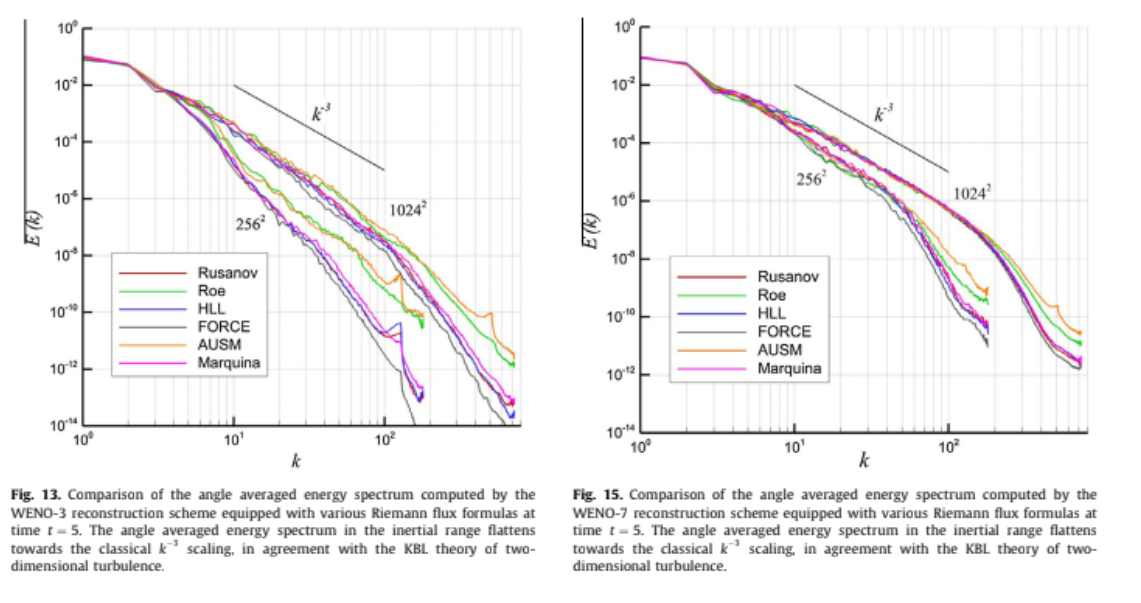
\includegraphics[width=\columnwidth]{ttk11.PNG}
 \caption{ Traitement traditionnel en aéronautique sur l'énergie en fonction du
nombre d'onde.}
 \label{fig:sample}
\end{figure}


\begin{figure}[H]
 \centering % avoid the use of \begin{cener}...\end{center} and use \centering
instead (more compact)
 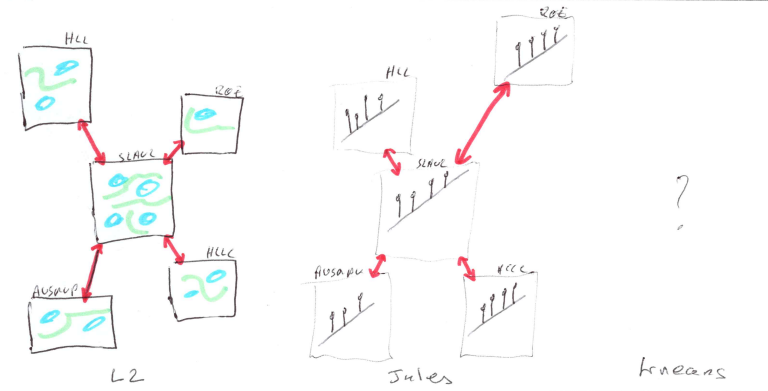
\includegraphics[width=\columnwidth]{ttk2.PNG}
 \caption{Visualisation de la distance L2, les flèches en rouge représentent la
distance entre deux simulation (VTI) à t2(figure de gauche)\\
 Visualisation de la distance topologique, les flèches en rouge représentent la
distance topologique (méthode de Jules) entre deux simulation (Diagrammes de
persistance) à t2(figure du milieu)\\
 Visualisation de la distance topologique, les flèches en rouge représentent la
distance topologique (méthode Kmeans) entre deux simulation (Diagrammes de
persistance) à t2(figure de droite)}
 \label{fig:sample}
\end{figure}


\begin{figure}[H]
 \centering % avoid the use of \begin{center}...\end{center} and use \centering
instead (more compact)
 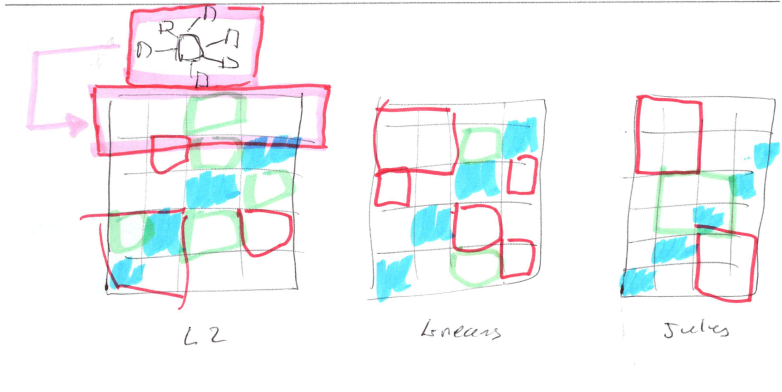
\includegraphics[width=\columnwidth]{ttk3.PNG}
 \caption{Visualisation de la distance L2, les flèches en rouge représentent la
distance entre deux simulation (VTI) à t2(figure en haut à gauche). Matrice de
distance pour la L2 avec les simulations à t2(en bas à gauche). Les carrés en
rouge représentent les clusters de la méthode L2.\\
 Visualisation de la distance topologique, les flèches en rouge représentent la
distance topologique (méthode de Jules) entre deux simulation (Diagrammes de
persistance) à t2(figure en haut du milieu).
 Matrice de distance pour la méthode de Jules avec les simulations à t2(en bas à
gauche). Les carrés en rouge représentent les clusters de la méthode Kmeans.\\
 Visualisation de la distance topologique, les flèches en rouge représentent la
distance topologique (méthode Kmeans) entre deux simulation (Diagrammes de
persistance) à t2(figure en haut à droite).
  Matrice de distance pour la méthode de Jules avec les simulations à t2(en bas
à gauche). Les carrés en rouge représentent les clusters de la méthode de
Jules.\\}
 \label{fig:sample}
\end{figure}


\begin{figure}[H]
 \centering % avoid the use of \begin{center}...\end{center} and use \centering
instead (more compact)
 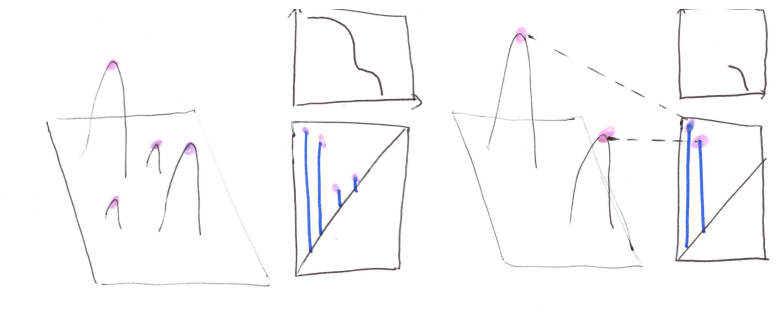
\includegraphics[width=\columnwidth]{ttk4.PNG}
 \caption{Les points critiques en rose sont les maximas. Simulation non filtrée
d'un KHI avec son diagramme de persistance (en bas à gauche) et sa courbe de
persistance (en haut à gauche).\\
 Les points critiques en rose sont les maximas. Simulation filtrée d'un KHI avec
son diagramme de persistance (en bas à droite) et sa courbe de persistance (en
haut à droite).}
 \label{fig:sample}
\end{figure}


\begin{figure}[H]
 \centering % avoid the use of \begin{center}...\end{center} and use \centering
instead (more compact)
 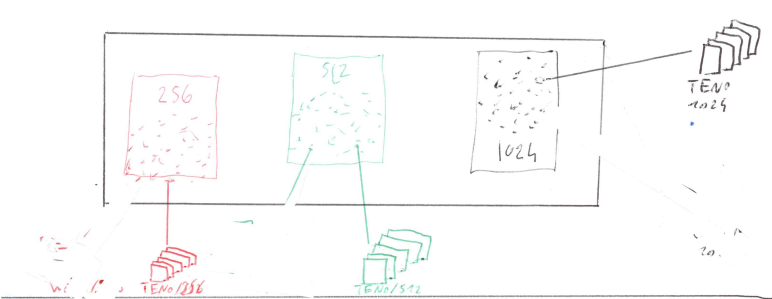
\includegraphics[width=\columnwidth]{ttk7.PNG}
 \caption{Nuage de points (ensemble 60*60), clusterisation par résolution avec
visualisation de certains VTI.}
 \label{fig:sample}
\end{figure}


\begin{figure}[H]
 \centering % avoid the use of \begin{center}...\end{center} and use \centering
instead (more compact)
 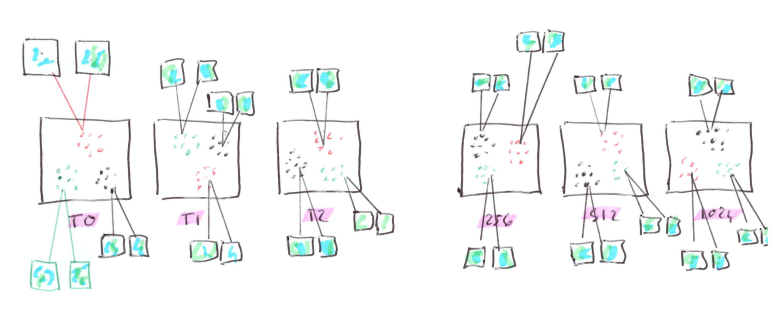
\includegraphics[width=\columnwidth]{ttk6.PNG}
 \caption{Nuage de points à t0,t1 et t2 (ensemble 60*60) avec visualisation de
certains VTI( figure de gauche).\\
 Nuage de points en fonction des résolutions: 256, 512, 1024 (ensemble 60*60)
avec visualisation de certains VTI(figure de droite).}
 \label{fig:sample}
\end{figure}

\begin{figure}[H]
 \centering % avoid the use of \begin{center}...\end{center} and use \centering
instead (more compact)
 \includegraphics[width=\columnwidth]{numerical_study.png}
 \caption{Etude numerique en CFD}
 \label{fig:sample}
\end{figure}


\begin{table}[!ht]
    \centering
    \begin{tabular}{|l|l|l|l|l|}
    \hline
        Schemes & Orders & Meshes & Solvers & Simulation times in seconds \\ \hline
        TENO & 5 & 256*256 & SLAU2 & 140.744 \\ \hline
        TENO & 5 & 256*256 & AUSM$^+$-UP & 212.350 \\ \hline
        TENO & 5 & 256*256 & Roe & 138.090 \\ \hline
        TENO & 5 & 256*256 & HLLC & 216.531 \\ \hline
        TENO & 5 & 256*256 & HLL & 132.921 \\ \hline
        TENO & 5 & 512*512 & SLAU2 & 1235.121 \\ \hline
        TENO & 5 & 512*512 & AUSM$^+$-UP & 786.758 \\ \hline
        TENO & 5 & 512*512 & Roe & 634.823 \\ \hline
        TENO & 5 & 512*512 & HLLC & 1273.546 \\ \hline
        TENO & 5 & 512*512 & HLL & 1119.895 \\ \hline
        TENO & 5 & 1024*1024 & SLAU2 & 10272.841 \\ \hline
        TENO & 5 & 1024*1024 & AUSM$^+$-UP & 5823.188 \\ \hline
        TENO & 5 & 1024*1024 & Roe & 5390.730 \\ \hline
        TENO & 5 & 1024*1024 & HLLC & 5612.924 \\ \hline
        TENO & 5 & 1024*1024 & HLL & 5187.889 \\ \hline
        TENO & 7 & 256*256 & SLAU2 & 189.150 \\ \hline
        TENO & 7 & 256*256 & AUSM$^+$-UP & 185.992 \\ \hline
        TENO & 7 & 256*256 & Roe & 189.150 \\ \hline
        TENO & 7 & 256*256 & HLLC & 267.585 \\ \hline
        TENO & 7 & 256*256 & HLL & 89.920 \\ \hline
        TENO & 7 & 512*512 & SLAU2 & 805.142 \\ \hline
        TENO & 7 & 512*512 & AUSM$^+$-UP & 786.758 \\ \hline
        TENO & 7 & 512*512 & Roe & 1674.321 \\ \hline
        TENO & 7 & 512*512 & HLLC & 773.146 \\ \hline
        TENO & 7 & 512*512 & HLL & 1622.587 \\ \hline
        TENO & 7 & 1024*1024 & SLAU2 & 13165.878 \\ \hline
        TENO & 7 & 1024*1024 & AUSM$^+$-UP & 6779.093 \\ \hline
        TENO & 7 & 1024*1024 & Roe & 6320.002 \\ \hline
        TENO & 7 & 1024*1024 & HLLC & 6491.327 \\ \hline
        TENO & 7 & 1024*1024 & HLL & 6186.092 \\ \hline
        WENO-Z & 5 & 256*256 & SLAU2 & 107.150 \\ \hline
        WENO-Z & 5 & 256*256 & AUSM$^+$-UP & 110.780 \\ \hline
        WENO-Z & 5 & 256*256 & Roe & 108.424 \\ \hline
        WENO-Z & 5 & 256*256 & HLLC & 105.91 \\ \hline
        WENO-Z & 5 & 256*256 & HLL & 98.779 \\ \hline
        WENO-Z & 5 & 512*512 & SLAU2 & 456.877 \\ \hline
        WENO-Z & 5 & 512*512 & AUSM$^+$-UP & 974.777 \\ \hline
        WENO-Z & 5 & 512*512 & Roe & 914.106 \\ \hline
        WENO-Z & 5 & 512*512 & HLLC & 443.987 \\ \hline
        WENO-Z & 5 & 512*512 & HLL & 391.781 \\ \hline
        WENO-Z & 5 & 1024*1024 & SLAU2 & 13165.878 \\ \hline
        WENO-Z & 5 & 1024*1024 & AUSM$^+$-UP & 3977.280 \\ \hline
        WENO-Z & 5 & 1024*1024 & Roe & 3665.727 \\ \hline
        WENO-Z & 5 & 1024*1024 & HLLC & 3844.873 \\ \hline
        WENO-Z & 5 & 1024*1024 & HLL & 3351.741 \\ \hline
        WENO-Z & 7 & 256*256 & SLAU2 & 134.924 \\ \hline
        WENO-Z & 7 & 256*256 & AUSM$^+$-UP & 142.729 \\ \hline
        WENO-Z & 7 & 256*256 & Roe & 127.671 \\ \hline
        WENO-Z & 7 & 256*256 & HLLC & 138.541 \\ \hline
        WENO-Z & 7 & 256*256 & HLL & 123.721 \\ \hline
        WENO-Z & 7 & 512*512 & SLAU2 & 1181.648 \\ \hline
        WENO-Z & 7 & 512*512 & AUSM$^+$-UP & 603.104 \\ \hline
        WENO-Z & 7 & 512*512 & Roe & 547.285 \\ \hline
        WENO-Z & 7 & 512*512 & HLLC & 588.874 \\ \hline
        WENO-Z & 7 & 512*512 & HLL & 516.925 \\ \hline
        WENO-Z & 7 & 1024*1024 & SLAU2 & 10164.932 \\ \hline
        WENO-Z & 7 & 1024*1024 & AUSM$^+$-UP & 10095.930 \\ \hline
        WENO-Z & 7 & 1024*1024 & Roe & 9488.464 \\ \hline
        WENO-Z & 7 & 1024*1024 & HLLC & 9195.901 \\ \hline
        WENO-Z & 7 & 1024*1024 & HLL & 8620.182 \\ \hline
    \end{tabular}
    \caption{Table of simulation times}
\end{table}
